\section{六个质量区作为比较坐标}\label{sec:1-4}

上一节说明，给定一个形状图像，还要知道占据、耦合与响应，才能讨论核怎样运动。把这些问题放回不同原子核中，会看到哪些相似之处，又会在哪里遇到差别？本论文选取 $A\approx 60$、$80$、$100$、$130$、$160$、$190$ 六个质量区作为比较坐标。质量数是质子与中子的总数，能够帮助定位案例，却没有规定价核子的轨道、激发态构型或运动模式。$A\approx 130$ 是重要研究锚点；其它区域使这里的解释能够接受不同微观条件和实验探针的检验。

\subsection{六个入口，各自增加什么信息}\label{sec:1-4-1}

选择案例的依据是它能使哪个问题更清楚。讨论电荷关联时，可以比较寿命给出的跃迁强度与库仑激发约束的矩阵元网络；讨论取向运动时，则要把准粒子组态、能带连接和电磁响应放在一起。表~\ref{tab:1-4-six-regions}列出第~4~章的主要入口，其中电四极跃迁简称 $E2$。每行对应特定核素和测量范围，不把一个代表案例概括为整个区域的性质。

\begin{table}[htbp]
\centering
\small
\caption{六个质量区结构演化比较的主要入口（非全区代表性统计）、实验探针与证据边界}\label{tab:1-4-six-regions}
\begin{tabularx}{\textwidth}{p{2.0cm}p{4.8cm}X}
\toprule
质量区 & 代表案例与探针（主要入口，非全区代表性统计） & 比较价值与限制 \\
\midrule
$A\approx 60$ & $^{64}\mathrm{Ge}$；敲出反应布居后的反冲距离寿命与 $E2$ & 用态间强度检验集体描述；表中静四极矩是理论输出~\cite{doctoral-r1-g26-starosta-2007-64ge-rdm-e2} \\
$A\approx 80$ & $^{74}\mathrm{Kr}$、$^{76}\mathrm{Kr}$；多步库仑激发 & 对角矩与带间连接增加混合信息；内禀形状指认仍有条件~\cite{doctoral-r1-g27-clement-2007-prc-krypton-coulex} \\
$A\approx 100$ & $^{98}\mathrm{Zr}$；反冲距离寿命与衰变分支 & 比较基态和激发结构的连接；$E2$ 提取采用外部分支比~\cite{doctoral-r1-g28-singh-2018-98zr-lifetimes} \\
$A\approx 130$ & $^{133}\mathrm{Ce}$；$\gamma$ 符合、角关联和相对跃迁信息 & 比较不同组态的候选伙伴带；该文未取得候选带寿命~\cite{ayangeakaa-2013-evidence-multiple-chiral-doublet-bands-133ce} \\
$A\approx 160$ & $^{163}\mathrm{Lu}$；多角度线形寿命及带内、带间 $E2$ & 为摆动图像增加绝对强度约束；采用分支、混合比及构型映射须保留~\cite{campaign-g07-gorgen-2004-163lu-quadrupole-moments} \\
$A\approx 190$ & 偶偶核 $^{182\text{--}188}\mathrm{Hg}$；低能库仑激发 & 检查平缓主连接下的结构变化；对角项宽误差与空项限制解释~\cite{doctoral-r1-g31-bree-2014-prl112-coulex-182-188hg} \\
\bottomrule
\end{tabularx}
\end{table}

这些入口的差别也体现了证据层次。$^{64}\mathrm{Ge}$ 的寿命与 $E2$ 可以约束集体关联，但计算给出的反号静四极矩，不能改称测得了形状共存。Kr 的多步过程同时涉及多个态的连接和对角项，比单条跃迁提供更多信息，几何解释仍需考虑态混合。$^{98}\mathrm{Zr}$ 则把问题推进到同一核内不同结构之间：通往基态与激发态的强度为何不同，模型怎样连接这些态？到高自旋的 Ce 和 Lu，比较又加入了组态与取向的作用。Hg 的两态混合分析则提醒我们，一条主连接变化不大，未必意味着波函数没有重组。

例如，$^{133}\mathrm{Ce}$ 的原文用能带关系和跃迁比比较手征解释，寿命缺口限制的是绝对强度检验，不能拿邻核寿命补成实测。$^{163}\mathrm{Lu}$ 则有新的线形寿命，但由它导出的多个电磁量共享分支或多极混合比输入，比较时需保留这些依赖。这两类信息的作用不同，不宜按支持某种解释的条目多少计票。

\begin{figure}[htbp]
\centering
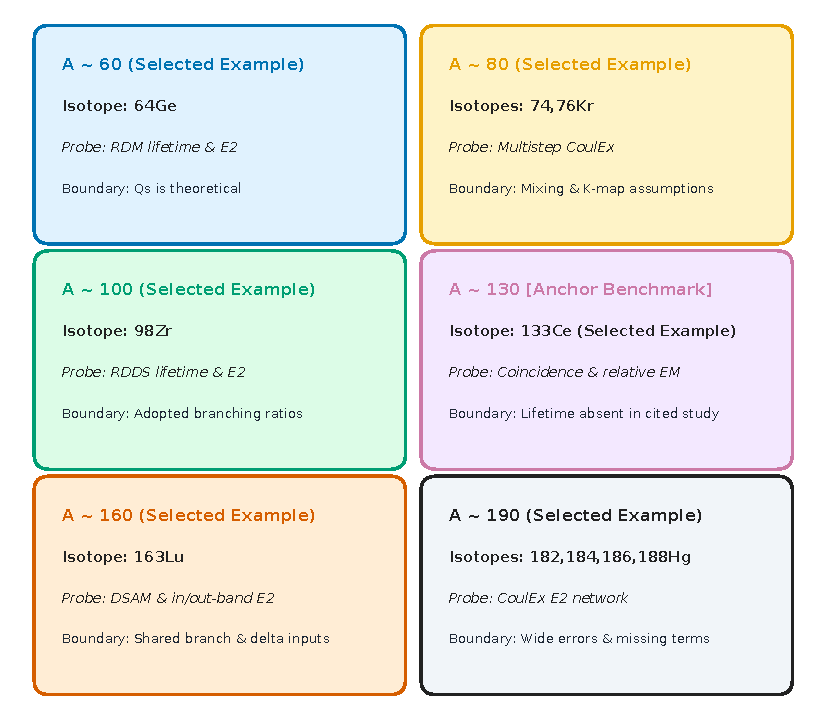
\includegraphics[width=.92\textwidth]{Img/six-region-map.pdf}
\caption{六个典型质量区结构演化、电磁探针与动力学机制比较坐标概念示意图。}\label{fig:six-region-map}
\end{figure}

\subsection{跨区比较要保留哪些条件}\label{sec:1-4-2}

质量数相近，费米面附近可用的轨道却可能不同。某个轨道在一核中主要以价粒子参与运动，在另一核中可能更适合用空穴描述；占据的变化又会影响四极耦合。奇粒子的加入、配对关联和核芯极化，也可能改变角动量怎样分配。这些才是比较相似能带时需要追问的条件。把``另一区也有近邻带''作为线索是有价值的，进一步讨论相同机制，则要检查相关组态能否形成、怎样耦合以及相应波函数的预言。

还要分清比较的是哪一种形状量和哪一种动力学量。库仑激发中的电荷矩阵元、模型势面的形变极小、转动惯量和带间跃迁，承担不同作用。即使电荷关联接近，势面的软硬、质量参数和激发次序也未必相同。$^{163}\mathrm{Lu}$ 的跃迁四极矩还经过顺排构型的映射，不能直接替代另一核的完整核芯响应。跨区比较因此需要对齐态的自旋、宇称、跃迁方向与所用算符，同时区分模型输入、拟合量和用于检验的观测，而不是给所有核设同一形变角或混合比界线。

这也限定了相邻主题之间的关系。Kr 的低自旋电荷结构不能代证 Br 的手征或八极性质；Zr 的结构演化不能概括同在 $A\approx 100$ 的 Mo、Ru；Hg 的低自旋网络也不能充当 Ir、Os 全部高自旋态的固定核芯。它们可以提供比较问题和分析方法，但各自的轨道占据、态连接与探针仍需独立建立。同一区域允许多种组态和运动，同一种现象也可能跨区出现；区域名称并没有替这些条件作出判断。

\subsection{未见的结构与尚未覆盖的窗口}\label{sec:1-4-3}

比较图上某类结构的空白，首先需要说明实验看到了哪里。反应可能难以产生目标核，或未有效布居所需的自旋和组态；级联馈送会改变各态的可见强度。即使有关态已经布居，很弱的退激分支、探测效率、本底以及时间接受度，也可能使连接跃迁难以分辨。反冲距离法利用飞行与减速过程取得时间信息，厚靶线形法则结合阻止过程拟合寿命，两者的可用窗口和输入依赖并不相同。一个实验未能取得寿命，也不意味着已有能谱和相对跃迁信息失去研究价值。

实验未观测与模型未得到稳定解，回答的同样是不同问题。前者需要交代搜索和接受度，后者依赖所用相互作用、坐标与近似。若某一区已有有用案例，另一区尚无对应信息，可以据此提出测量或计算的问题；在补齐相关条件前，既不能由空白推出不存在，也不能把跨区类比写成新模式已经发现。

六区地图因此保持开放。八极关联、异能态与弱衰变等两翼主题，可以在各自的态、算符和衰变通道条件下提供互补约束，其具体论证将在第~4~章展开。后文先建立占据、配对、形状和响应的机制，再逐例回到这张地图，比较哪些认识能够迁移，哪些差别需要新的观测解释。
